\chapter{Observations,Results and Challenges}

Critical phenomena in gravitational collapse are most clearly understood in spherical symmetry, where the approach to the critical regime is comparatively straightforward. In this case, the field equations reduce to a system of coupled one-dimensional partial differential equations, which can be solved with relatively high numerical accuracy. Indeed, in the pioneering work of Matthew Choptuik \cite{choptuik_1993}, the critical parameter was tuned to nearly machine precision, reaching approximately 15 decimal places.

However, once symmetry assumptions are relaxed, the problem becomes significantly more challenging. In the literature, studies of axisymmetric vacuum collapse typically achieve only about 5–7 digits of precision in tuning the critical parameter. This limitation arises both from the increased computational difficulty of solving multidimensional partial differential equations and from the intrinsic nature of critical phenomena, which involve the development of increasingly fine spatial and temporal structures near the threshold of black hole formation.

For the family of initial data considered in this work, the best-tuned critical parameter is found to be $(p^* = 4.110 \pm 0.003)$. Despite this comparatively modest level of tuning, we are able to extract a critical exponent of approximately $( \gamma \approx 0.55 \pm 0.32 )$, demonstrating the robustness of the scaling behaviour even without extremely fine-tuned initial data.

The quoted uncertainty in the critical parameter arises from the inability to unambiguously distinguish between subcritical and supercritical evolution within this narrow region of parameter space. In particular, near the threshold, small variations in the parameter lead to qualitatively different outcomes, and within our numerical resolution this transition cannot be resolved more precisely. This limitation propagates into the determination of the scaling exponent, contributing to the relatively large uncertainty in ($\gamma$).
\begin{figure}[!hbt]
    \centering
    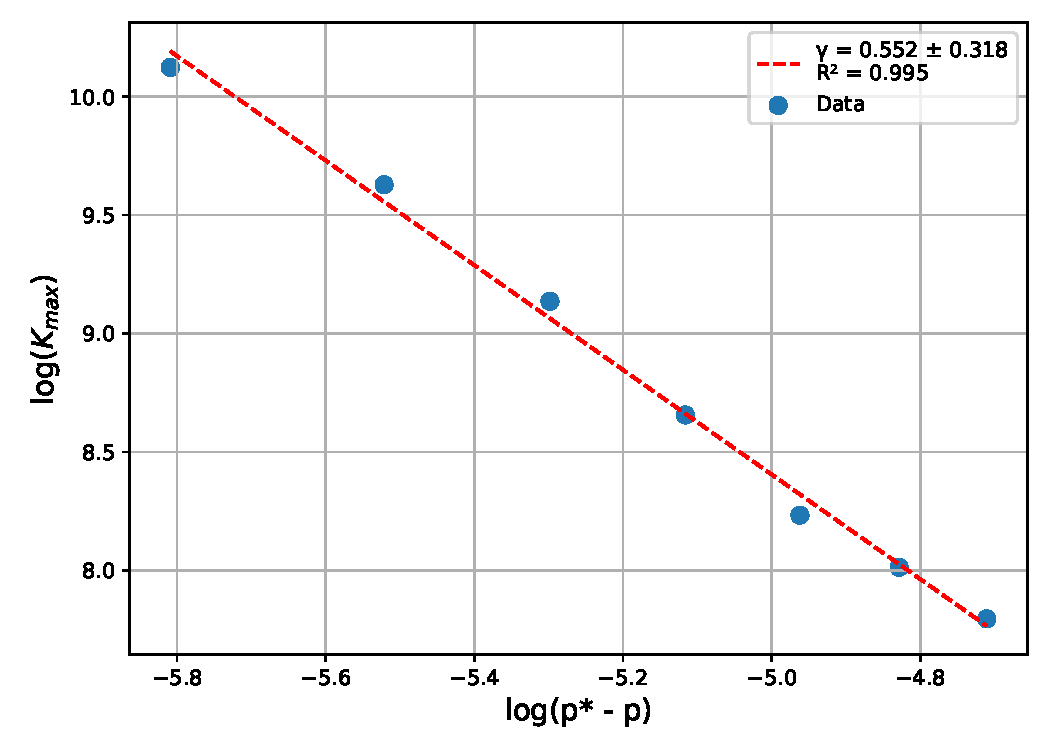
\includegraphics[scale=0.6]{../notebooks/plusfamily.pdf}
    \caption{Log--log plot of the maximum Kretschmann scalar $K_{\max}$ in subcritical evolutions as a function of $(p^* - p)$. Each data point corresponds to an independent simulation, with typical computational cost of $\sim 4000$ core-hours per run. The approximate linear behaviour supports the expected power-law scaling $K_{\max} \sim (p^* - p)^{-4\gamma}$ near criticality.}
\end{figure}

For the current family that we have chosen, we see a $R^2$ goodness of fit value of 0.995 which gives an additional assurance that there indeed exists some linear scaling even at this level of tuning.



But in this regard, more work needs to be done to tune more into the critical regime and investigate the critical phenomena (Presence of self-similiar structures and so on).

For example, as the parameter is tuned closer to the critical value, the evolution exhibits increasingly pronounced oscillatory features in the curvature, suggestive of the onset of echoing behaviour. These structures appear as repeated, self-similar peaks in the Kretschmann scalar as a function of proper time. However, due to the limited level of tuning and numerical resolution in the present simulations, these features cannot be conclusively identified as true discrete self-similarity. Achieving a more definitive verification would require finer tuning of the critical parameter and higher resolution to resolve the increasingly small spacetime scales involved.

\begin{figure}[!!hbt]
    \centering
    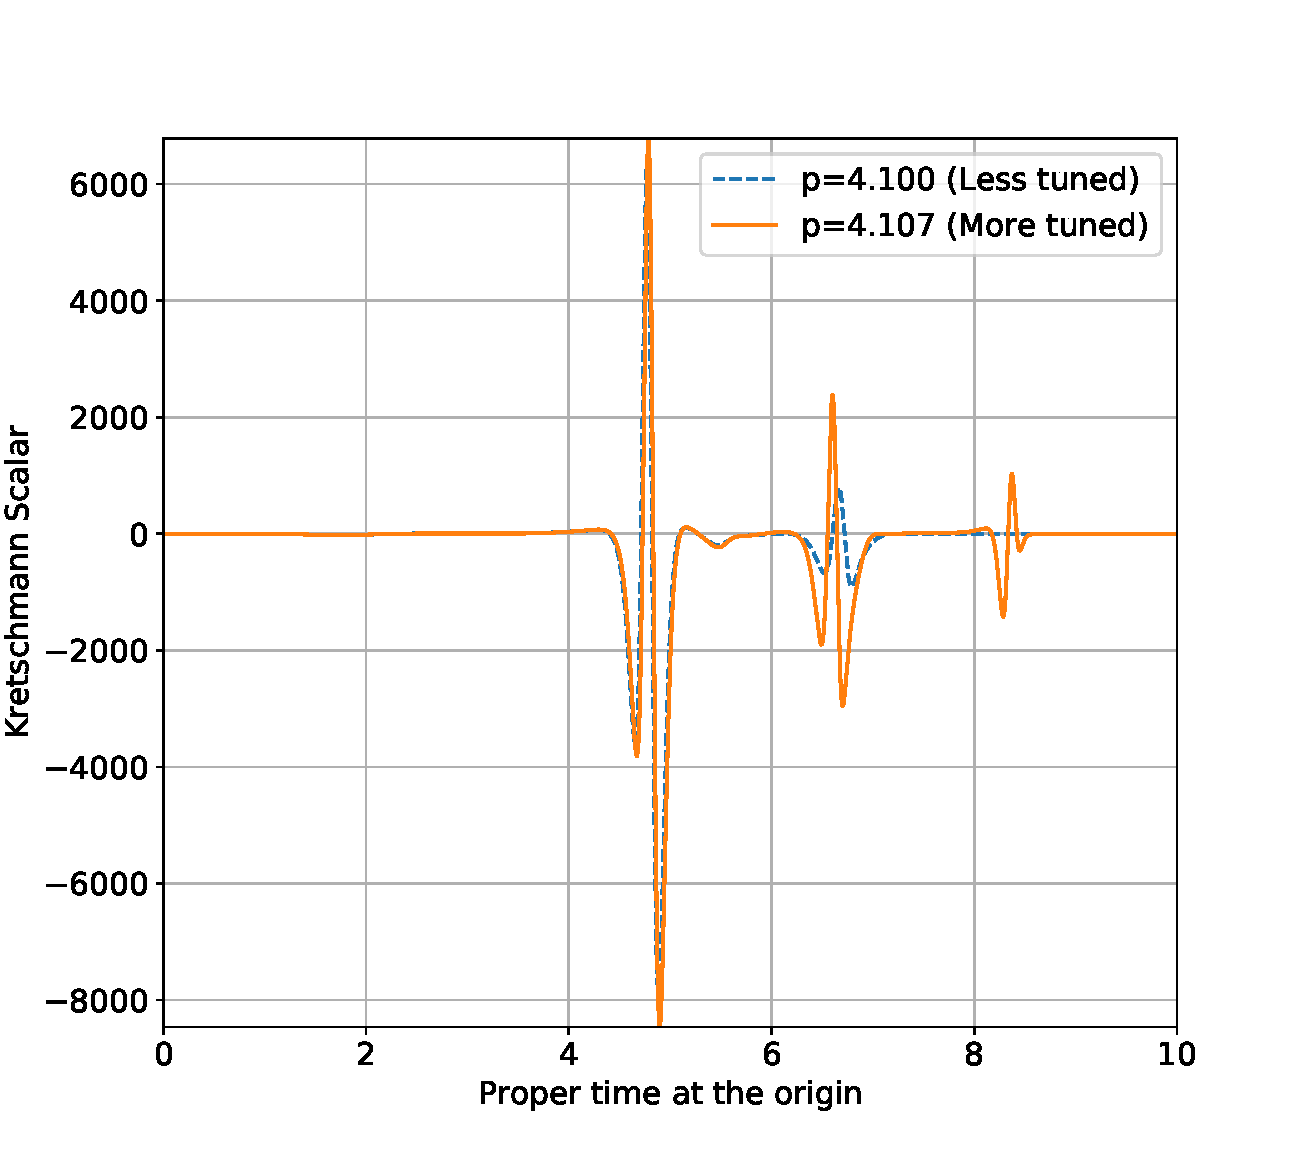
\includegraphics[scale=0.6]{../figures/feature.pdf}
    \caption{Log--log plot of the maximum Kretschmann scalar $K_{\max}$ in subcritical evolutions as a function of $(p^* - p)$. Each data point corresponds to an independent simulation, with typical computational cost of $\sim 4000$ core-hours per run. The approximate linear behaviour supports the expected power-law scaling $K_{\max} \sim (p^* - p)^{-4\gamma}$ near criticality.}
    \label{feature}
\end{figure}


\textbf{But what makes tuning and classifying spacetimes difficult?}

As the critical threshold is approached, it becomes increasingly difficult to classify a given evolution as subcritical or supercritical. In particular, near-critical evolutions may:

\begin{enumerate}
\item not exhibit clear dispersal of curvature to spatial infinity,
\item not form an apparent horizon detectable by standard horizon-finding tools,
\end{enumerate}

thereby making the outcome ambiguous within finite numerical resolution. This could be attributed to certain reasons as to why.

\section*{Development of Coordinate Pathologies}



\subsection*{Courant Condition and Resolution Limits}

As we approach the critical regime, the solution develops structure on increasingly small spatio-temporal scales. This imposes a fundamental restriction on the timestep through the Courant – Friedrichs – Lewy (CFL) condition, which is required for the stability of explicit numerical schemes.

The Courant condition states that the numerical domain of dependence must include the physical domain of dependence. For a hyperbolic system with characteristic speed $v_{\max}$, this leads to the condition
\[
\Delta t \leq C \frac{\Delta x}{v_{\max}},
\]
where $C < 1$ is the Courant factor determined by the numerical scheme.

This condition has important consequences near criticality. To resolve the features \texttt{BAMPS} uses Adaptive Mesh Refinement (AMR) which adjusts the spatial grid sizes to capture the dynamics that happen in smaller and smaller scales. As finer spatial resolution ($\Delta x \to 0$) is required to resolve the small-scale features that emerge, the timestep must also decrease proportionally. Consequently, the computational cost increases significantly, since the number of timesteps required scales inversely with $\Delta t$. With our current computational resources we were only able to tune to about 3 decimal places due to that reason.

Additionally, the dynamics of critical phenomenon is in such a way as we tune towards the threshold of collapse, the evolution resembles each other to even more duration of evolution until the solution "chooses" an end point, be it a singular spacetime or dispersion. So essentially we will have to evolve more as we tune the parameter more to reach the critical regime.



Therefore, the combination of shrinking physical scales and the CFL constraint severely limits how close one can tune to the critical parameter in multidimensional simulations. This is one of the primary reasons why achieving high precision in non-symmetric critical collapse is significantly more challenging than in spherical symmetry.





\begin{figure}
    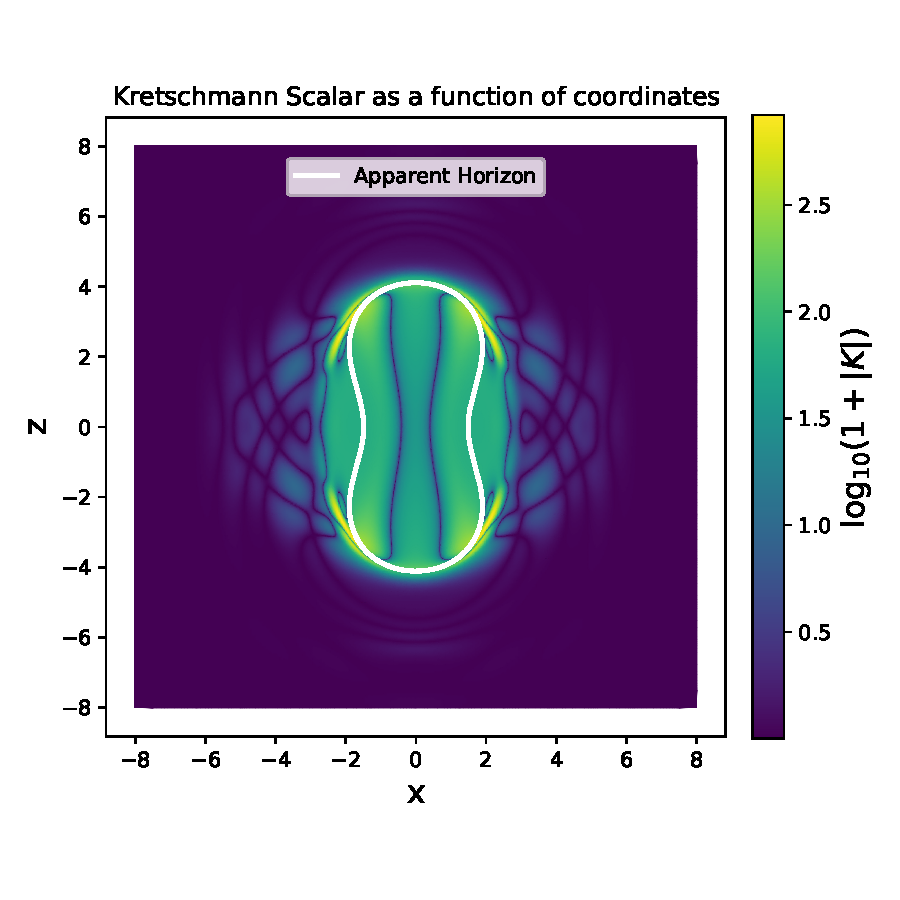
\includegraphics[scale=0.8]{../notebooks/figure.pdf}
    \caption{}
\end{figure}

\subsubsection{Harmonic Horizon Marching Gauge}
\label{HHMG}
Since GR has an intrinsic gauge freedom built into it, it will be reflected when we do simulations using NR as well. Hence we will have to choose a gauge but in the case of simulations they are chosen by the stability it confers to the simulations.

In \texttt{BAMPS}, the usual gauge that we use is HDWG (Harmonic Gauge). Here the evolution equations for the lapse becomes,

\[
\mathcal{L}_n \log \alpha = - (H_n +K)
\]

where $H_n$ is the free choosable function which only contains the metric and not its derivatives.

Inorder the push the lapse to 1 we add an extra term into the harmonic function in such a way that it adds a term $\eta_{hm}(\alpha-1)$ into the evolution equation for lapse

\[
\partial_t \alpha -\beta^i \partial_i \alpha= -\alpha^2(H_n + K)
\]

The extra term that in $H_n$ is $\eta_{hm} \alpha^{-2} (\alpha-1)$

\[
\partial_t \alpha -\beta^i \partial_i \alpha= -(\eta_{hm} (\alpha-1) + \alpha^2 K)
\]

So in $H_a$ an extra term of $-\eta_{hm} \alpha^{-2} (\alpha - 1) n_a$ is added

So New $H_0=.... + \eta_{hm} \alpha^{-1} (\alpha-1)$

\[
\partial_t H_0 = +\eta_{hm} \alpha^{-2} \partial_t \alpha
\]

\[
\partial_i H_0 = +\eta_{hm} \alpha^{-2} \partial_i \alpha
\]